\begin{frame}
    \frametitle{Cámara Time of Flight}
    \note{https://en.wikipedia.org/wiki/Time-of-flight_camera}
    \scriptsize

    \begin{figure}[!h]
        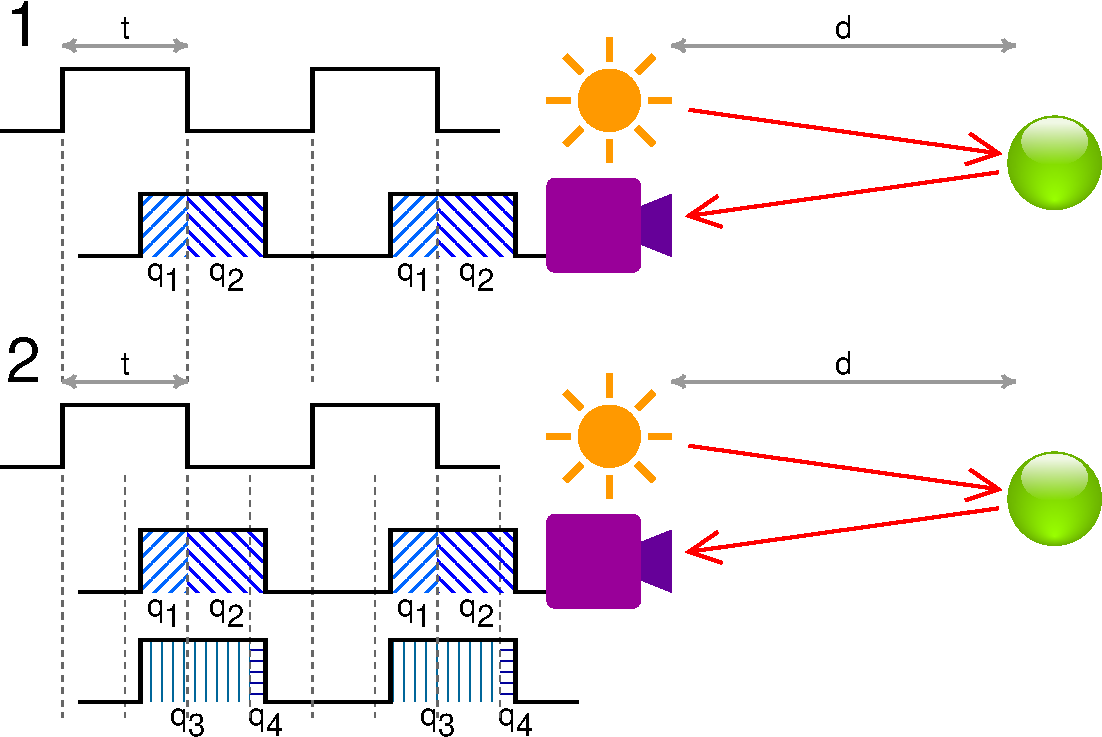
\includegraphics[width=0.4\columnwidth]{images/time_of_flight_camera.pdf}
    \end{figure}
    
    \begin{block}{Principio de funcionamiento}
        Funciona de manera similar a un lidar con la ventaja de que toda la escena 3D se captura al mismo tiempo y que no hay partes móviles. Este dispositivo utiliza una fuente de luz infrarroja modulada para determinar la distancia de cada píxel de un sensor Photonic Mixer Device (PMD).
        
        En el método basado en Pulsos (1), la ditancia es
        \begin{equation*}
            d = d\frac{c t}{2} \dfrac{q_{2}}{q_{1} + q_{2}}
        \end{equation*}
        
        donde $c$ es la velocidad de la luz, $t$ es la longitud del pulso, $q_{1}$ es la carga acumulada en el píxel cuando se emite luz y $q_{2}$ es la carga acumulada cuando no se emite.
        
        En el método de onda continua (2):
        
        \begin{equation*}
            d = \frac{c t}{2\pi} \arctan \dfrac{q_{3} - q_{4}}{q_{1} - q_{2}}
        \end{equation*}        
    \end{block}
    
    \begin{itemize}
        \item Esteroceptivo
        \item Activo
        \item La precisión suele estimarse en un $\SI{1}{\percent}$ de la distancia medida, suelen tener un frame rate de unos $\SI{160}{\hertz}$
        \item La luz del entorno puede quemar la imagen (requiere píxeles con buen rango dinámico)
    \end{itemize}
    
\end{frame}